\PassOptionsToPackage{svgnames}{xcolor}
\documentclass[12pt]{article}



\usepackage[margin=1in]{geometry}  
\usepackage{graphicx}             
\usepackage{amsmath}              
\usepackage{amsfonts}              
\usepackage{framed}   
\usepackage{mathtools}            
\usepackage{amssymb}
\usepackage{array}
\usepackage{amsthm}
\usepackage[nottoc]{tocbibind}
\usepackage{bm}
\usepackage{enumitem}


\DeclareMathOperator{\Tr}{Tr}
 \newcommand{\im}{\mathrm{i}}
  \newcommand{\diff}{\mathrm{d}}
  \newcommand{\col}{\mathrm{Col}}
  \newcommand{\row}{\mathrm{R}}
  \newcommand{\kerne}{\mathrm{Ker}}
  \newcommand{\nul}{\mathrm{Null}}
  \newcommand{\nullity}{\mathrm{nullity}}
  \newcommand{\rank}{\mathrm{rank}}
  \newcommand{\Hom}{\mathrm{Hom}}
  \newcommand{\id}{\mathrm{id}}
  \newcommand{\ima}{\mathrm{Im}}
  \newcommand{\lcm}{\mathrm{lcm}}
  \newcommand{\diag}{\mathrm{diag}}
  \newcommand{\expec}{\mathrm{E}}
  \newcommand{\var}{\mathrm{var}}
  \newcommand{\cov}{\mathrm{cov}}
  \newcommand{\inv}{^{-1}}
  \newcommand{\str}{^\ast}
  \newcommand{\corr}{\mathrm{corr}}
  \newcommand{\Poi}{\mathrm{Poisson}}
  \newcommand\norm[1]{\left\lVert#1\right\rVert}
\setlength{\parindent}{0cm}
\setlength{\parskip}{0em}
\newcommand{\Lim}[1]{\raisebox{0.5ex}{\scalebox{0.8}{$\displaystyle \lim_{#1}\;$}}}
\newtheorem{definition}{Definition}[section]
\newtheorem{theorem}{Theorem}[section]
\newtheorem{notation}{Notation}[section]
\theoremstyle{definition}
\DeclareMathOperator{\arcsec}{arcsec}
\DeclareMathOperator{\arccot}{arccot}
\DeclareMathOperator{\arccsc}{arccsc}
\DeclareMathOperator{\spn}{Span}
\setcounter{tocdepth}{1}
\begin{document}

\title{PYP Answer - MA3269 AY1617Sem2}
\author{Ma Hongqiang}
\maketitle
\begin{enumerate}
  \item \begin{enumerate}
    \item $r_f=0$ since CML has $\mu$ intercept of $0$.
    \item We have in general, $\sigma^2=A(\mu-\mu_g)^2+\sigma_g^2$, where $A$ is some constant to be determined. By GMVP, we have
    \[
\sigma^2=A(\mu-\frac{1}{6})^2+\frac{1}{12}
    \]
    And by portfolio $x$, we have
    \[
\frac{1}{4}=A(0-\frac{1}{6})^2+\frac{1}{12}
    \]
    Solving, $A=6$.
    Therefore, $\sigma^2=A(\mu-\frac{1}{6})^2+\frac{1}{12}$.\\Rearranging,
    \[
\mu=\frac{1}{6}\pm\sqrt{\frac{1}{6}\sigma^2-\frac{1}{72}}
    \]
    \item From (ii), we can easily write down $\sigma=\sqrt{6}(\mu-\frac{1}{6})$.
    \item From (ii), we can solve $\mu_y = \frac{1}{3}$.
    \item From (ii), we have the following equations
    \[
    \begin{cases}
    \frac{a}{ac-b^2}=6\\
    \frac{b}{a}=\frac{1}{6}\\
    \frac{1}{a}=\frac{1}{12}
    \end{cases}
\]
Solving, we have
\[
\begin{cases}
a=12\\
b=2\\
c=\frac{1}{2}
\end{cases}
\]
Then, $\mu_m=\frac{c-r_fb}{b-r_fa}=\frac{c}{b}=\frac{1}{4}$ and $\sigma_m^2=\frac{c}{b^2}=\frac{1}{8}$.
\item Using the definition of beta, $\beta_p = \frac{\mu_p-r_f}{\mu_m-r_f}$, we have
\[
\beta_g = \frac{2}{3}\;\;\beta_m = 1\;\;\beta_x = 0\;\;\beta_y = \frac{4}{3}
\]
Therefore, the required portfolio beta is
\[
\beta = \frac{1}{4}(\beta_g+\beta_m+\beta_x+\beta_y)=\frac{1}{4}(\frac{2}{3}+1+0+\frac{4}{3})=\frac{9}{8}
\]
\item 
\begin{align*}
\corr(r_y, r_m)&=\frac{\sigma_{ym}}{\sigma_y\sigma_m}\;\;\text{by definition of correlation}\\
&=\frac{\frac{\mu_y}{\mu_m}\sigma_m^2}{\sigma_y\sigma_m}\;\;\text{by CAPM}\\
&=\frac{2\sqrt{2}}{3}
\end{align*}
  \end{enumerate}
\item \begin{enumerate}
\item \begin{enumerate}
\item The payoff table is 
\begin{table}[h]
\centering
\begin{tabular}{|c|c|c|c|}
\hline
&$0\leq S_T< K_1$&$K_1\leq S_T<K_2$&$S_T\geq K_2$\\\hline
Payoff&0&$S_T-K_1$&$K_2-K_1$\\\hline
\end{tabular}
\end{table}
The graph has turning point $(K_1, 0)$, $(K_2, K_2-K_1)$ and is piecewise linear. 
\begin{figure}[h]
\centering
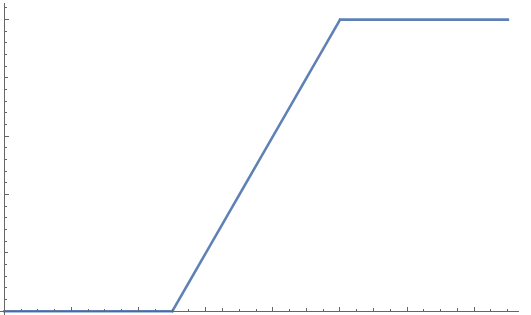
\includegraphics[width = 0.3\textwidth]{2_1.png}
\end{figure} 
\item One possible portfolio would be 1 long $K_1$-put, 1 short $K_2$-put and $e^{-rT}(K_2-K_1)$ risk-free asset.
\end{enumerate}
\item\begin{enumerate}
\item $n_1=2\;\;n_2=3\;\;n_3=3\;\;K=108$
\item It is a piecewise linear function with turning points (80,60), (90,30), (100,30), (108,54) and (120,78).
\end{enumerate} 
\item We have $S_0 = 10, S_1^u = 11, S_1^d = 9.5$. Therefore, $u=1.1, d=0.95$ and $F_1^u = 3, F_1^d = 0.225$.\\Also, we identify that $r=0.06$ and $\delta t = \frac{1}{12}$.\\
By single-period binomial model, we have
\[
q=\frac{e^{r\delta t}-d}{u-d}=0.366750139
\]
and hence
\[
F_0=e^{-r\delta t}(qF_1^u+(1-q)F_1^d)=1.237
\]
\end{enumerate}
\item \begin{enumerate}
\item\begin{enumerate}
\item 
\begin{align*}
U(C(x))&=\expec[U(w_0+X)]\\
\ln C(x)&=\frac{1}{2}\ln(1+ax)+\frac{1}{2}\ln(1-bx)\\
\ln(C(x)^2) &= \ln[(1+ax)(1-bx)]\\
C(x)&=[(1+ax)(1-bx)]^\frac{1}{2}
\end{align*}
The last square root opertion retains the positive root since $\min(w_0+X)=\min(1-bx)\geq 0$.
\item Differentiate $C(x)$, we yield
\[
\frac{\diff C(x)}{\diff x}=\frac{1}{2}\frac{1}{C(x)}(-2abx-b+a)
\]
Obviously the first and second fraction are both positive. For the third term, note that, when $a\leq b$,
\begin{align*}
&0<bx<1\\
0<2abx<2a\\
&-2abx-b+a<0-b+a+1\leq -b+b=0
\end{align*}
Therefore, the last term is negative so the derivative is negative, and hence $C(x)$ is a strictly decreasing function of $x$.
\item The trader will avoid the lottery when $C(x)<w_0=1$. Therefore we need
\[
0<(1+ax)(1-bx)<1\Rightarrow \frac{a-b}{ab}<x<\frac{1}{b}.
\]
\item Let the derivative to equual 0. We need $2abx+b-a=0$. Therefore, $x=\frac{a-b}{2ab}:=\xi$.\\
Also, we check easily check taht for all $x>\xi$, the derivative is negative and for all $x<\xi$, derivative is positive. Therefore, $x=\xi$ is indeed the maximum.\\
Then, since $\xi<\frac{a-b}{ab}$, the trader will indeed play the lottery.
\end{enumerate}
\item \begin{enumerate}
\item For this subquestion, $x$ is a variable and is dropped for simplicity. Since $U=U_1U_2^{-1}$, 
\[
\frac{\diff U}{\diff x}=(U_1^\prime\circ U_2^{-1})(U_2^{-1})^\prime
\]
and
\begin{align*}
\frac{\diff^2U}{\diff x^2}&=-(U_1''\circ U_2^{-1})[(U_2^{-1})']^2+(U_1^\prime\circ U_2^{-1})(U_2^{-1})''\\
&=\frac{-U_1''(t)U_1'(t)}{(U_2'(t))^2U_1'(t)}+\frac{-U_2''(t)U_1'(t)}{(U_2'(t))^2U_2'(t)}\\
&=RHS
\end{align*}
\item Since $R_2(t)<R_1(t)$ for all $t>0$, we indeed have a concave $U$.
Next, since $U_2$ is positive and increasing $U_2^{-1}$ is also positive and increasing and its composite with an positive and increasing $U_1$ is also positive and increasing.\\
Therefore, $U$ is indeed a concave untility function.
\end{enumerate}
\end{enumerate}
\begin{enumerate}
  \item We first calculate $\sigma_y^2 = \mathbf{w}_y^\text{T}\mathbf{C}\mathbf{w}_y$.
  \begin{align*}
  \sigma_y^2&=(\alpha\frac{\mathbf{C}^{-1}\mathbf{\mu}}{b}+(1-\alpha)\frac{\mathbf{C}^{-1}\mathbf{1}}{a})^\text{T}\mathbf{C}(\alpha\frac{\mathbf{C}^{-1}\mathbf{\mu}}{b}+(1-\alpha)\frac{\mathbf{C}^{-1}\mathbf{1}}{a})\\
  &=\frac{\alpha^2}{b^2}c+\frac{1-\alpha^2}{a}
  \end{align*}
  Similarly, $\sigma_x^2 = \frac{\alpha}{b}\mu_y+\frac{1-\alpha}{a}\;\;(\#)$.\\
  Next, $\mu_y = \mu^\text{T}\mathbf{w}_y = \alpha\frac{c}{b}+(1-\alpha)\frac{b}{a}$. Subsitute into $(\#)$ yields the result.
  \item Note that $\rho_{px}=\frac{\sigma_{px}}{\sigma_p\sigma_x}$. Therefore, we need to show
  \[\frac{\sigma_{px}}{\sigma_p}=\frac{\gamma \sigma_y^2+(1-\gamma)\sigma_g^2}{\sqrt{\gamma^2\sigma_y^2+(1-\gamma^2)\sigma_g^2}}
  \]
  We first calculate $\sigma_p^2$.
  \begin{align*}
  \sigma_p^2&=(\gamma\mathbf{w}_y+(1-\gamma)\mathbf{w}_g)^\text{T}\mathbf{C}(\gamma\mathbf{w}_y+(1-\gamma)\mathbf{w}_g)\\
  =\gamma^2\sigma_y^2+(1-\gamma^2)\sigma_g^2
  \end{align*}
  So we have verified the denominator. Next we show the nominator matches:
  \begin{align*}
  \sigma_{px}&=\mathbf{w}_p\mathbf{C}\mathbf{w}_x\\
  &=\gamma\sigma^2_y+(1-\gamma)\sigma_g^2
  \end{align*}
  We want to maximise $\rho_{px}$. By computing the derivative, we have
  \[
\frac{\diff \rho_{px}}{\diff \gamma}=\frac{(b(1-\gamma)+a\gamma)(2a\gamma-2b\gamma)}{2c(a\gamma^2+b(1-\gamma^2))^\frac{3}{2}}+\frac{a-b}{c\sqrt{a\gamma^2+b(1-\gamma^2)}}
  \]
where $a=\sigma_y^2$, $b=\sigma_g^2$ and $c=\sigma_x$.
Letting the derivative to equal 0, we have $\sigma = 1$. Therefore, the highest correlation is attained when $r_p=r_y$, i.e., by portfolio y.
\item Indeed, we have $w_a = w_x-w_y$ and $w_b = w_y-w_g$.
\item By one fund theorem, we have $\mathbf{w}_z = \alpha\mathbf{w}_m$. Therefore, $\sigma_{xz} = \alpha\sigma_{xm}$.\\
Since $\rho_{xz}=\frac{\sigma_{xz}}{\sigma_x\sigma_z}$. We will show the claim if we show that $\sigma_{xz}=\sigma_{z}^2$.\\
Note that $\sigma_z^2 = \alpha^2\sigma_m^2$. So we need to show $\sigma_{xm}=\alpha\sigma_{m}^2$.\\
This is indeed the case. Since $\beta_x=\beta_z=\alpha\beta_m=\alpha$. So we have our result.
\end{enumerate}
\end{enumerate}
\end{document}